%\newpage
\subsection*{Statement of authorship}
\renewcommand{\arraystretch}{1.5}
\begin{tabular}{m{0.25\textwidth} m{0.67\textwidth}}
    \hline \hline Paper title & Optimization of the Magnetic Field Produced by Frustum Permanent Magnets for Single Magnet and Planar Halbach Array Configurations \\ \hline
    Publication status & Published \\ \hline
    Publication details & J. L. G. O’Connell, W. S. P. Robertson, and B. S. Cazzolato, ``Optimization of the Magnetic Field Produced by Frustum Permanent Magnets for Single Magnet and Planar Halbach Array Configurations,'' in IEEE Transactions on Magnetics, vol. 57, no. 8, Aug. 2021, doi: 10.1109/TMAG.2019.2942538. \\ \hline \hline
\end{tabular}

\vfill

\subsection*{Principal author}
\begin{tabular}{p{0.25\textwidth} m{0.67\textwidth}}
    \hline \hline Name & James O'Connell \\ \hline
    Contribution & \begin{itemize}
        \setlength\itemsep{-2mm}
        \item[-] Idea conceptualisation
        \item[-] Review of relevant literature
        \item[-] Performing a parametric optimisation of the geometry of a frustum magnet to maximise the field strength at a particular point using the field equations from Chapter \ref{chap:paper2}, including writing and testing MATLAB code to run the optimisation routine
        \item[-] Defining the geometry and topology of a planar magnet array consisting of frustum magnets
        \item[-] Performing a parametric optimisation on the magnet array geometry to maximise a cost function, including writing and testing MATLAB code to run the optimisation routine
        \item[-] Generalising the parametric optimisation to include a wider range of geometric configurations
        \item[-] Wrote manuscript draft and created all figures
        \item[-] Finalisation of article
        \item[-] Preparation and submission for publication, including author correspondence
    \end{itemize} \\ \hline
    Percentage & 90\% \\ \hline
    Certification & This paper reports on original research conducted by the author during the period of Higher Degree by Research candidature and is not subject to any obligations or contractual agreements with a third party that would constrain its inclusion in this thesis. The author listed above is the primary author of this paper. \\ \hline
    Signature & \begin{tabular}{m{45mm} m{10mm} m{20mm}}
    \vspace{0.5mm}\includegraphics[width=0.3\textwidth]{jamesSignature.PNG} & Date: & 8 Dec 2021
    \end{tabular} \\ \hline
\end{tabular}

\vfill
    
\subsection*{Co-author contributions}
By signing this statement of authorship, each author certifies that:
\begin{enumerate}
    \item the candidate's stated contribution to the publication is accurate (as detailed above);
    \item permission is granted for the candidate to include the publication in the thesis; and
    \item the sum of all co-author contributions is equal to 100\% less the candidate's stated contribution.
\end{enumerate}
\begin{tabular}{m{0.25\textwidth} m{0.67\textwidth}}
    \hline \hline Name & Will Robertson \\ \hline
    Contribution & 5\% \\ \hline
    Signature & \vspace{2mm}\includegraphics[height=10mm]{willSig} \\  \hline
    Date & 16 Dec 2021 \\
    \hline \hline Name & Ben Cazzolato \\ \hline
    Contribution & 5\% \\ \hline
    Signature & \vspace{2mm} \includegraphics[height=10mm]{benSig} \\ \hline
    Date & 16 Dec 2021 \\
    \hline \hline \vfill
\end{tabular}
\renewcommand{\arraystretch}{1}
\newpage
%
\section*{\LARGE Optimisation of the magnetic field Produced by frustum permanent magnets for single magnet and planar Halbach array configurations}
James L.G. O'Connell, William S.P. Robertson, and Benjamin S. Cazzolato
\section*{Abstract}\addcontentsline{toc}{section}{\protect\numberline{}Abstract}\label{sec:p3abstract}
The potential benefits of frustum-shaped magnets over cuboidal magnets have been seldom studied. This paper compares these magnet shapes by optimising frustum geometry for both a single magnet and for a multi-magnet planar Halbach array to produce a desirable field\footnote{In this chapter, optimisation for a single magnet refers to maximising the field strength per unit magnet volume, and optimisation for an array refers to minimising the cost function defined in Equation (\ref{eqn:p3CostFunction})}. This field is compared to the equivalent field for optimised cuboidal magnets and differences quantified. A single magnet is considered, where the field strength above the centre of a magnet is maximised. If the field is measured close to the magnet surface, an optimised frustum magnet can produce a field stronger than an optimised cuboidal magnet. If the field is measured further from the magnet, there is little benefit in using a frustum magnet over a cuboid. Additionally, a planar magnet array is considered, in which the field strength and how closely the field resembled a sinusoidal profile are maximised. In this case, no significant benefit is observed using frustum magnets over cuboidal magnets.
\section{Introduction}\label{sec:p3introduction}
Cuboidal permanent magnets have been studied extensively in literature, with the first three-dimensional field equations derived in 1984 by \textcite{Akoun1984}. Since then, more general equations have been derived describing the fields produced by cuboidal magnets. \textcite{Bancel1999} showed that a cuboidal magnet is equivalent to a set of magnetic point charges located at the vertices when calculating the field, and \textcite{Ravaud2009} presented field equations for a cuboidal magnet with an arbitrary magnetisation direction. Other studies have explored the forces between two parallel cuboidal magnets \cite{Akoun1984,Janssen2009a}, the torque between two parallel cuboidal magnets \cite{Allag2009,Janssen2011,Janssen2010}, and the force between cuboidal magnets under rotations about a single axis \cite{Dam2016}.

The geometry of a permanent magnet has a considerable effect on the field it produces, and as such, modifying the geometry of a six-sided magnet from a conventional cuboid may lead to a more desirable field. By angling two pairs of opposite faces of a cuboid, a six-sided frustum is created, such as the one shown in Figure \ref{fig:p3myFrustum}. Due to the angled faces being trapezial instead of rectangular, the field equations become significantly more difficult to derive, and thus frustum magnets have been seldom studied. However, several approaches have been used to derive field equations produced by polyhedral magnets \cite{Compter2010,Fabbri2008,Janssen2010a,Janssen2009,OConnell2020,Rubeck2013,OConnell2020a}, which can be applied to frustum magnets.

In addition to single magnets, considerable research has been conducted on magnet arrays. In particular, the linear Halbach array, first theorised by \textcite{Mallinson1973}, has been studied extensively. In recent years, this has lead to further investigation into planar Halbach arrays for use in planar actuators, for which studies have modelled the magnetic field using cuboidal magnets \cite{Boeij2006,Rovers2012} and triangular prismatic magnets \cite{Cho2001} with magnetisations parallel to a principal axis. Further studies have been conducted to optimise the magnetic field produced by planar Halbach arrays using cuboidal magnets \cite{Huang2008,Jansen2008} and triangular or trapezoidal prismatic magnets \cite{Cho2002,Peng2013}. \textcite{Min2010} has considered cuboidal magnets with magnetisations which are not parallel to a principal axis, leading to a field with a stronger \(z\)-component with smaller high-order harmonics. However, all aforementioned studies are limited to magnets with faces either parallel or orthogonal to the \(z\)-axis; i.e. the normal vector of every magnet face is parallel to the \(z\) axis or lies in the \(XY\)-plane. There exists little-to-no research on magnets with faces rotated about the \(x\)- or \(y\)-axes.

This paper applies previous polyhedral magnet field equations to frustum magnets in order to explore potential advantages they have over cuboidal magnets. In Section \ref{sec:p3frustumField}, the method used to calculate the magnetic field produced by a frustum magnet is outlined. This methodology is applied to a square-based right frustum permanent magnet in Section \ref{sec:p3pyramidFrustum}, where the geometry is varied to optimise the magnetic field strength at a point above the magnet. Section \ref{sec:p3planarArray} presents a two-dimensional permanent magnet Halbach array, where the magnetic field is optimised by varying the magnet geometry. These geometries are compared to the equivalent cuboidal geometries, and any advantage in frustum magnets quantified.
\section{Magnetic field produced by a pyramid frustum magnet}\label{sec:p3frustumField}
To calculate the magnetic field produced by a frustum permanent magnet, it is assumed ideal, with constant uniform magnetisation \(\mathbf{M}\) and a relative permeability \(\mu_r\) of unity. Under this assumption, a simplified version of the magnetic charge model outlined by \textcite{Furlani2001} can be applied to calculate the magnetic field \(\mathbf{B}\) at a point \(\mathbf{x}\), given by
\begin{equation}
\mathbf{B}\left(\mathbf{x}\right) = \frac{\mu_0}{4\pi} \oint_S \left( \mathbf{M} \cdot \hat{\mathbf{n}} \right) \frac{\mathbf{x} - \mathbf{x}'}{\left| \mathbf{x} - \mathbf{x}' \right| ^3} ds' \text{,}
\label{eqn:p3chargeModel}
\end{equation}
where \(\mu_0\) is the permeability of free space, \(\mathbf{M}\) is the magnetisation vector, \(\hat{\mathbf{n}}\) is the outward-facing unit normal vector of the magnet surface \(S\), \(\mathbf{x}'\) is a point on \(S\), and \(ds'\) is a surface element of \(S\).

This paper uses the field solution presented by the current authors \cite{OConnell2020a}, in which the magnet is deconstructed into each of its polygonal facets. Consider the rectangular pyramid frustum permanent magnet shown in Figure \ref{fig:p3myFrustum}. This is composed of two parallel rectangular surfaces and four trapezial surfaces joining the rectangles with symmetry in the \(XZ\) and \(YZ\) planes. One rectangular surface lies on the \(XY\)-plane, with the origin placed at the centre of the surface. The magnetic field is given by the sum of the field contributions from each of the rectangles \(\mathbf{B}_{\text{rect,}i}\) and trapezia \(\mathbf{B}_{\text{trap,}j}\),
\begin{align}
\mathbf{B} = \sum_{i=1}^2 \mathbf{B}_{\text{rect,}i} + \sum_{j=1}^4 \mathbf{B}_{\text{trap,}j} \text{.}
\end{align}
The following sections outline the methodology for calculating the field.
\begin{figure}
	\centering
	\def\lim{13}

\tdplotsetmaincoords{70}{45}
\begin{tikzpicture}[scale=0.115,tdplot_main_coords]

% Define coordinates:
\coordinate(ppb) at (15,20,-20);
\coordinate(pnb) at (15,-20,-20);
\coordinate(nnb) at (-15,-20,-20);
\coordinate(npb) at (-15,20,-20);
\coordinate(ppt) at (5,10,0);
\coordinate(pnt) at (5,-10,0);
\coordinate(nnt) at (-5,-10,0);
\coordinate(npt) at (-5,10,0);

% Fill in polygons:
\filldraw[fill=white] (ppt) -- (pnt) -- (nnt) -- (npt) -- cycle;
\filldraw[fill=white] (ppt) -- (ppb) -- (pnb) -- (pnt) -- cycle;
\filldraw[fill=white] (pnt) -- (nnt) -- (nnb) -- (pnb) -- cycle;

% Axes:
\draw[->] (0,0,0) -- (\lim,0,0);
\draw[->] (0,0,0) -- (0,\lim,0);
\draw[->] (0,0,0) -- (0,0,\lim);
\node(xaxis) at (\lim+2,0,0) {\(x\)};
\node(yaxis) at (0,\lim+2,0) {\(y\)};
\node(zaxis) at (0,0,\lim+2) {\(z\)};

\end{tikzpicture}
	\caption{A pyramid frustum created by joining two parallel rectangular surfaces with four quadrilateral surfaces. The rectangular surfaces are parallel to the \(XY\)-plane, with the origin at the centre of the top rectangular surface.}
	\label{fig:p3myFrustum}
\end{figure}

\subsection{Field solution for a magnetically charged trapezium}
Consider the magnetically charged trapezium depicted in Figure \ref{fig:p3trapezium} with surface charge \(\sigma = \mathbf{M} \cdot \hat{\mathbf{n}}\). It lies parallel to the \(\tilde{X}\tilde{Y}\)-plane with a \(\tilde{z}\)-coordinate of \(z'\) and the parallel edges being parallel to the \(\tilde{y}\)-axis. The magnetic field \(\mathbf{B}\left(\tilde{\mathbf{x}}\right) = \left[ B_{x}, B_{y}, B_{z} \right]\) due to this trapezium at the point \(\tilde{\mathbf{x}} = \left(\tilde{x}, \tilde{y}, \tilde{z}\right)\) is presented by the current authors \cite{OConnell2020a} and is given by
\begin{align}\label{eqn:p3fieldequation}
B_{\tilde{x}}\left(\tilde{\mathbf{x}}\right) &= \frac{\mu_0 \sigma}{4\pi} \sum_{p=1}^2 \sum_{q=1}^2 \Bigg[ \left( -1 \right) ^{p+q} \Bigg( \ln \left( T_{pq} \right) - \frac{m_p}{\sqrt{1+m_p^2}} \ln \left(S_{pq}\right) \Bigg) \Bigg] \nonumber \\
B_{\tilde{y}}\left(\tilde{\mathbf{x}}\right) &= \frac{\mu_0 \sigma}{4\pi} \sum_{p=1}^2 \sum_{q=1}^2 \left[ \left( -1 \right)^{p+q} \frac{1}{\sqrt{1+m_p^2}} \ln \left( S_{pq} \right) \right] \\
B_{\tilde{z}}\left(\tilde{\mathbf{x}}\right) &= \frac{\mu_0 \sigma}{4\pi} \sum_{p=1}^2 \sum_{q=1}^2 \Bigg[ \left( -1 \right) ^{p+q} \arctan \left( U_{pq} \right) \Bigg] \text{,} \nonumber
\end{align}
where
\begin{align}\label{eqn:p3intermediatevars}
\begin{split}
X &= x_q - \tilde{x} \\
Y &= c_p + m_px_q - \tilde{y} \\
Z &= z' - \tilde{z} \\
R_{pq} &= \sqrt{X^2 + Y^2 + Z^2} \\
S_{pq} &= X + m_pY + \sqrt{1+m_p^2}R_{pq} \\
T_{pq} &= R_{pq} + Y \\
U_{pq} &= \frac{m_p\left(X^2+Z^2\right)-XY}{ZR_{pq}} \text{.}
\end{split}
\end{align}
This solution can be applied to each of the six surfaces of the frustum permanent magnet, as described in Sections \ref{sec:p3rectFaces} and \ref{sec:p3trapFaces}.
\begin{figure}
	\centering
	\def\lim{10}

\begin{tikzpicture}[scale=0.5]
	\coordinate(negx) at (-1,0);
	\coordinate(posx) at (\lim+2,0);
	\coordinate(negy) at (0,-5);
	\coordinate(posy) at (0,7);
	
	\coordinate(TL) at (1,6);
	\coordinate(BL) at (1,-4);
	\coordinate(TR) at (\lim,1);
	\coordinate(BR) at (\lim,-1);
	
	\draw[<->] (negx) -- (posx);
	\draw[<->] (negy) -- (posy);
	\filldraw[fill=black!5, fill opacity=0.8] (BL) -- (BR) -- (TR) -- (TL) -- cycle;
	
	\draw[dashed] (BL) -- (1,-5.5);
	\node(x1) at (1.25,-6) {\(\tilde{x} = x_1\)};
	\draw[dashed] (BR) -- (\lim,-5.5);
	\node(x2) at (\lim+0.25,-6) {\(\tilde{x} = x_2\)};
	\node(m1c1) at (6,-3.5) {\(\tilde{y}=m_1\tilde{x}+c_1\)};
	\node(m2c2) at (6,5) {\(\tilde{y}=m_2\tilde{x}+c_2\)};
	\node(x) at (\lim+2.5,0) {\(\tilde{x}\)};
	\node(y) at (0,7.4) {\(\tilde{y}\)};
\end{tikzpicture}
	\caption{A trapezial surface parallel to the \(XY\)-plane. It has two parallel edges, \(x = x_1\) and \(x = x_2\), and two nonparallel edges joining them, \(y = m_1x+c_1\) and \(y = m_2x+c_2\).}
	\label{fig:p3trapezium}
\end{figure}

\subsection{Rectangular faces}\label{sec:p3rectFaces}
The field solution for the two rectangular faces is a simplified case of the trapezium. Both rectangular surfaces are already parallel to the \(XY\)-plane, and two edges parallel to the \(y\)-axis, so no rotation is necessary. Since two edges are parallel to the \(x\)-axis, \(m_p = 0\) and Equation (\ref{eqn:p3fieldequation}) is simplified. This simplification is equivalent to the expressions seen in studies on cuboidal magnets \cite{Akoun1984,Ravaud2009a}. The point \(\mathbf{x}\) and geometric parameters can be substituted into Equation (\ref{eqn:p3fieldequation}) to obtain the magnetic field for each of the rectangular surfaces,
\begin{align}
\mathbf{B}_{\text{rect,}i} = \mathbf{B}\left(\mathbf{x}\right) \text{.}
\end{align}

\subsection{Trapezial faces}\label{sec:p3trapFaces}
The fields produced by the four trapezial surface are more difficult to evaluate than those produced by the rectangular surfaces since they require rotation and \(m_p \neq 0\) in general. However, since each of the four trapezia have normal vectors orthogonal to either the \(x\)- or \(y\)-axes, the rotation matrices are simple. If the trapezia are numbered as shown in Figure \ref{fig:p3numberedTrapezia}, then the rotation matrices corresponding to each trapezium are given by
\begin{figure}
	\centering
	\def\lim{5}

\tdplotsetmaincoords{0}{0}
\begin{tikzpicture}[scale=0.115,tdplot_main_coords]

% Define coordinates:
\coordinate(ppb) at (15,20,-20);
\coordinate(pnb) at (15,-20,-20);
\coordinate(nnb) at (-15,-20,-20);
\coordinate(npb) at (-15,20,-20);
\coordinate(ppt) at (5,10,0);
\coordinate(pnt) at (5,-10,0);
\coordinate(nnt) at (-5,-10,0);
\coordinate(npt) at (-5,10,0);

% Draw shape:
\draw (ppt) -- (pnt) -- (nnt) -- (npt) -- cycle;
\draw (ppb) -- (pnb) -- (nnb) -- (npb) -- cycle;
\draw (ppt) -- (ppb);
\draw (pnt) -- (pnb);
\draw (nnt) -- (nnb);
\draw (npt) -- (npb);

% Draw some lines of symmetry
\draw[dashed,black!30] (-20,0,0) -- (20,0,0);
\draw[dashed,black!30] (0,-25,0) -- (0,25,0);

% Number the trapezia:
\node[circle,draw,fill=white](1) at (11,0,0) {1};
\node[circle,draw,fill=white](2) at (0,16,0) {2};
\node[circle,draw,fill=white](3) at (-11,0,0) {3};
\node[circle,draw,fill=white](4) at (0,-16,0) {4};

% Axes:
\draw[->] (0,0,0) -- (\lim,0,0);
\draw[->] (0,0,0) -- (0,\lim,0);
%\draw[->] (0,0,0) -- (0,0,\lim);
\node(xaxis) at (\lim+2,0,0) {\(x\)};
\node(yaxis) at (0,\lim+2,0) {\(y\)};
%\node(zaxis) at (0,0,\lim+2) {\(z\)};



\end{tikzpicture}
	\caption{A pyramid frustum as viewed from the positive \(z\)-axis with the four angled surfaces numbered.}
	\label{fig:p3numberedTrapezia}
\end{figure}
\begin{align}
\begin{split}
R_1 &= \begin{bmatrix}
n_z & 0 & n_x \\
0 & 1 & 0 \\
-n_x & 0 & n_z
\end{bmatrix} \text{,}
\quad
R_2 = \begin{bmatrix}
0 & n_z & -n_y \\
-1 & 0 & 0 \\
0 & n_y & n_z
\end{bmatrix} \text{,} \\[3mm]
R_3 &= \begin{bmatrix}
n_z & 0 & -n_x \\
0 & 1 & 0 \\
n_x & 0 & n_z
\end{bmatrix} \text{,}
\quad
R_4 = \begin{bmatrix}
0 & -1 & 0 \\
n_z & 0 & n_y \\
-n_y & 0 & n_z
\end{bmatrix} \text{,}
\end{split}
\end{align}
where \(\hat{\mathbf{n}} = \left[ n_x, n_y, n_z \right]\) is the outward-facing unit normal vector of each trapezium.

The rotation matrix \(R_j\) defines a temporary coordinate system \(\left( \tilde{x}, \tilde{y}, \tilde{z} \right)\) in which the trapezium is parallel to the \(\tilde{X}\tilde{Y}\)-plane, allowing the use of Equation (\ref{eqn:p3fieldequation}). In this new coordinate system, the field point is given by \(\mathbf{x} R_j\) and the vertices of the trapezium in the new coordinate system can be similarly found by postmultiplying by \(R_j\). Once the field is calculated in the new coordinate system, it can be transformed back to the original coordinate system by postmultiplying by \(R_j^{-1}\). Thus, the field contribution of each trapezium is given by
\begin{equation}
\mathbf{B}_{\text{trap,}j} = \mathbf{B}\left( \mathbf{x} R_j \right) R_j^{-1} \text{.}
\end{equation}
\section{Maximising the field above a right pyramid frustum magnet}\label{sec:p3pyramidFrustum}
Consider the symmetric right square pyramid frustum, herein referred to as a right frustum, shown in Figure \ref{fig:p3squareFrustum}. It is composed of a pair of parallel squares centred on the \(z\)-axis joined by four identical trapezia. It has constant uniform magnetisation \(\mathbf{M} = \left[ 0, 0, M_z \right]\) and a relative permeability \(\mu_r\) of unity. The top surface has a side length of \(L\), the bottom surface has a side length of \(l\), and the slanted faces form an angle \(\theta\) with the bottom face. The volume of the frustum is given by
\begin{equation}
V = \frac{l-L}{6}\tan\theta \left( L^2 + lL+ l^2 \right) \text{,}
\end{equation}
and a length parameter\footnote{In this section, \(\upsilon\) is a length based on the volume, and is used to nondimensionalise lengths, allowing a dimensionless analysis.} \(\upsilon\) is defined as \(\upsilon = \sqrt[3]{V}\).

If the field is to be evaluated at any point on the \(z\)-axis, i.e. at a point \(\left(0,0,z\right)\), symmetry can be exploited and the field produced by the magnet can be evaluated with a single function, given by
\begin{figure}
	\centering
	

\begin{subfigure}[t]{\linewidth}

\centering
\tdplotsetmaincoords{70}{45}
\begin{tikzpicture}[scale=0.1,tdplot_main_coords]

% Define coordinates:
\coordinate(ppb) at (20,20,-20);
\coordinate(pnb) at (20,-20,-20);
\coordinate(nnb) at (-20,-20,-20);
\coordinate(npb) at (-20,20,-20);
\coordinate(ppt) at (10,10,0);
\coordinate(pnt) at (10,-10,0);
\coordinate(nnt) at (-10,-10,0);
\coordinate(npt) at (-10,10,0);

% Fill in polygons:
\filldraw[fill=white] (ppt) -- (pnt) -- (nnt) -- (npt) -- cycle;
\filldraw[fill=white] (ppt) -- (ppb) -- (pnb) -- (pnt) -- cycle;
\filldraw[fill=white] (pnt) -- (nnt) -- (nnb) -- (pnb) -- cycle;

% Axes:
\def\lim{13}
\draw[->] (0,0,0) -- (\lim,0,0);
\draw[->] (0,0,0) -- (0,\lim,0);
\draw[->] (0,0,0) -- (0,0,\lim);
\node(xaxis) at (\lim+2,0,0) {\(x\)};
\node(yaxis) at (0,\lim+2,0) {\(y\)};
\node(zaxis) at (0,0,\lim+2) {\(z\)};

\end{tikzpicture}

\subcaption{}
\label{subfig:p3frustum3d}

\end{subfigure}

\vspace{20pt}

\begin{subfigure}[t]{\linewidth}

\centering
\begin{tikzpicture}[scale = 0.2]

\def\LL{5}
\def\ll{10}
\def\hh{10}

% Define coordinates:
\coordinate(tl) at (-\LL,0);
\coordinate(tr) at (\LL,0);
\coordinate(bl) at (-\ll,-\hh);
\coordinate(br) at (\ll,-\hh);

% Draw shape
\draw (tl) -- (tr) -- (br) -- (bl) -- cycle;

% Draw axes
\def\arrowlim{7}
\draw[->] (0,0) -- (\arrowlim,0);
\draw[->] (0,0) -- (0,\arrowlim);
\node(x) at (\arrowlim+1,0) {\(x\)};
\node(z) at (0,\arrowlim+1) {\(z\)};

% Draw dimensions
\def\hoffset{12}
\draw[<->] (\hoffset,0) -- (\hoffset,-\hh);
\node(h) at (\hoffset+1,-5) {\(h\)};
\node(l) at (0,-\hh-1.5) {\(l\)};
\node(L) at (0,-1.5) {\(L\)};
\node(theta) at (-7.5,-8.5) {\(\theta\)};

% Draw an invisible line to centre the figure
\draw[<->,white] (-\hoffset-2,0) -- (-\hoffset-2,-\hh);

% Draw magnetisation vector
\draw[->,thick] (0,-8) -- (0,-4);
\node(M) at (1.5,-6) {\(\mathbf{M}\)};

\end{tikzpicture}

\subcaption{}
\label{subfig:p3frustumschematic}

\end{subfigure}


	\caption{Three-dimensional view (\subref{subfig:p3frustum3d}) and schematic (\subref{subfig:p3frustumschematic}) of a right square pyramid frustum permanent magnet with magnetisation vector \(\mathbf{M}\). The origin is located at the centre of the top surface and both rectangular surfaces are parallel to the \(XY\)-plane. The frustum has a nondimensional height \(h\), a top surface side length \(L\), and bottom surface side length \(l\). The four angled surfaces form an angle \(\theta\) with the bottom surface.}
	\label{fig:p3squareFrustum}
\end{figure}
\begin{align}
B_x = &\ 0 \nonumber \\
B_y = &\ 0 \nonumber \\
B_z = &\ \frac{\mu_0 M_z}{\pi} \left[ \arctan\left(\frac{L^2}{4zR_{0}}\right) - \arctan\left(\frac{l^2}{4\left(z+h\right)R_{1}}\right)\right. \nonumber \\
&\ +\left. \sum_{p=0}^1 \sum_{q=0}^1 \left(-1\right)^{p+q} \cos\theta \Big(\arctan\left(U_{pq}\right) \cos\theta    \Big.\right. \nonumber \\
&\qquad \ \left.\Big.  - \ln\left(T_{pq}\right)\sin\theta - \frac{\left(-1\right)^p\sin\theta}{\sqrt{1+\sec^2\theta}} \ln\left({S_{pq}}\right) \Big) \right] \text{,}
\end{align}
where
\begin{align*}
l_q &= L + 2hq\cot\theta \\
R_{q} &= \sqrt{\frac{l_q^2}{2}+\left(z+qh\right)^2} \\
S_{pq} &= l_q\cos\theta + \left(z+qh\right)\sin\theta + \sqrt{1+\cos^2\theta}R_{q} \\
T_{pq} &= R_{q} - \frac{\left(-1\right)^p l_q}{2} \\
U_{pq} &= \frac{\left(-1\right)^p\left(z+qh\right)}{R_{q}} \text{.}
\end{align*}
It should be noted that a cylindrical frustum can produce a stronger field than that of a rectangular frustum along the axis of symmetry. However, rectangular frusta have the ability to tessellate well (as discussed in Section \ref{sec:p3planarArray}), and as such only rectangular frusta are considered in this work.

A right frustum requires three parameters to fully describe the geometry. For a magnet with a given volume \(V\), the length dimensions can be normalised by the length parameter \(\upsilon\). Here, the normalised height \(h/\upsilon\) and wall angle \(\theta\) are varied for a frustum with volume \(V\). For each pair \((h/\upsilon,\theta)\), the magnetic field produced by the frustum was evaluated at the point \(\left( 0, 0, z/\upsilon\right)\) and normalised by the magnetisation strength of the magnet.

First, the field was evaluated at \(z/\upsilon = 0.1\) for all physically realisable pairs \(\left( h/\upsilon, \theta\right)\), where physically realisable refers to all lengths being positive and real, and a contour plot drawn in Figure \ref{subfig:p3centralField100}. The field is maximised by a frustum with a normalised height of \(h_\text{opt}/\upsilon = 0.95\) units and a wall angle of \(\theta_\text{opt} =\) \ang{57}. The equivalent optimal cuboidal magnet is found in the same way, but constraining the wall angle to \ang{90}. For \(z/\upsilon = 0.1\), the optimal frustum produces a field 12.6\% stronger than the optimal cuboid. Schematics of both the optimal frustum and optimal cuboid for \(z/\upsilon = 0.1\) are shown in Figure \ref{fig:p3optimalGeom_z_0_1}. This optimisation was repeated for a point \(z/\upsilon = 0.5\) units above the magnet (Figure \ref{subfig:p3centralField500}), resulting in an optimal frustum with \(h_\text{opt}/\upsilon = 0.83\) units and \(\theta_\text{opt} =\) \ang{94}. This optimal frustum is almost cuboidal in shape, leading to a field only 0.07\% stronger than the equivalent optimal cuboid.

To give an indication of optimal magnet shape, the \(z\)-field was calculated in the region above a cube magnet, shown in Figure \ref{fig:p3optimalFrusAndCube}. In addition, the optimal cuboid and frustum for \(z/\upsilon = 0.1\) were drawn, with a `+' sign representing the point at which the field is maximised. All three magnets have identical volumes and magnetisations, with the field calculated over the same region; only the shape of the magnet differs. It can be seen that the cube magnet has the weakest field strength at this point, with the optimal cuboid having a slightly stronger field. However, the optimal frustum `focuses' the flux through the top surface, leading to a larger magnetic field at the point of interest.
\begin{figure}
    \centering
	\begin{subfigure}{0.8\textwidth}
		\centering
		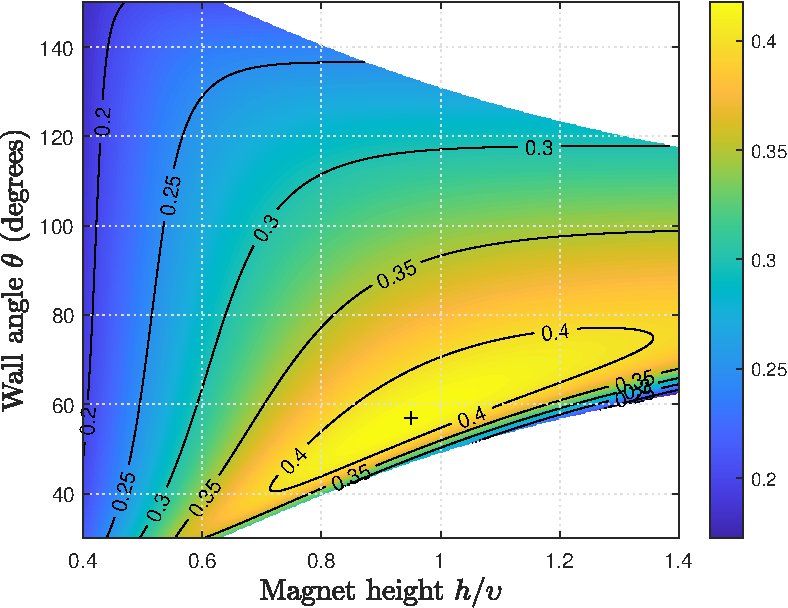
\includegraphics[width=\linewidth]{p3/p3FIG5a}
		\subcaption{}
		\label{subfig:p3centralField100}
	\end{subfigure}
	
	\begin{subfigure}{0.8\textwidth}
		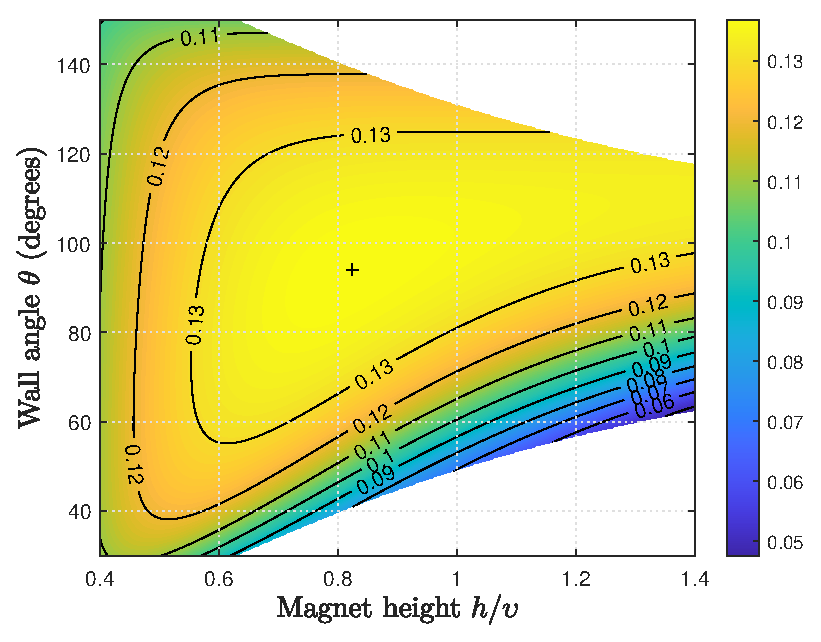
\includegraphics[width=\linewidth]{p3/p3FIG5b}
		\subcaption{}
		\label{subfig:p3centralField500}
	\end{subfigure}
	\caption{Normalised magnetic field strength \(z/\upsilon = 0.1\) (\subref{subfig:p3centralField100}) and \(z/\upsilon = 0.5\) (\subref{subfig:p3centralField500}) units above the centre of a right frustum magnet with a volume \(V\), a normalised height of \(h/\upsilon\) units and wall angle of \(\theta\) degrees. The global maxima \(\left( h_\text{opt}/\upsilon, \theta_\text{opt}\right)\) for each plot is highlighted with a `+', with the white regions indicating non-physical geometries.}
	\label{fig:p3centralField}
\end{figure}
\begin{figure}
	\centering
	

\begin{subfigure}[t]{0.45\linewidth}

\centering
\begin{tikzpicture}[scale = 0.3]

\def\LL{1}
\def\ll{4.5950}
\def\hh{5.5312}

% Define coordinates:
\coordinate(tl) at (-\LL,0);
\coordinate(tr) at (\LL,0);
\coordinate(bl) at (-\ll,-\hh);
\coordinate(br) at (\ll,-\hh);

% Draw shape
\draw (tl) -- (tr) -- (br) -- (bl) -- cycle;

% Draw dimensions
\def\hoffset{6}
\draw[<->] (-\hoffset,0) -- (-\hoffset,-\hh);
\node(h) at (-\hoffset-1.5,-2.7656) {0.951};
\draw[<->] (-\ll,-\hh-1.5) -- (\ll,-\hh-1.5);
\node(l) at (0,-\hh-2.5) {1.580};
\draw[<->] (-\LL,1.5) -- (\LL,1.5);
\node(L) at (0,2.5) {0.344};

\end{tikzpicture}

\subcaption{}
%\label{subfig:frustumschematic}

\end{subfigure}
~ \hfill ~
\begin{subfigure}[t]{0.45\linewidth}

\centering
\begin{tikzpicture}[scale = 0.3]
	
\def\LL{2.3647}
\def\ll{2.3647}
\def\hh{8.8066}

% Define coordinates:
\coordinate(tl) at (-\LL,0);
\coordinate(tr) at (\LL,0);
\coordinate(bl) at (-\ll,-\hh);
\coordinate(br) at (\ll,-\hh);

% Draw shape
\draw (tl) -- (tr) -- (br) -- (bl) -- cycle;

% Draw dimensions
\def\hoffset{5}
\draw[<->] (\hoffset,0) -- (\hoffset,-\hh);
\node(h) at (\hoffset+1.5,-4.4033) {1.514};
\draw[<->] (-\ll,-\hh-1.5) -- (\ll,-\hh-1.5);
\node(l) at (0,-\hh-2.5) {0.813};

% Draw an invisible line to centre the figure
%\draw[<->,white] (-\hoffset-2,0) -- (-\hoffset-2,-\hh);

\end{tikzpicture}

\subcaption{}
%\label{subfig:frustumschematic}

\end{subfigure}


	\caption{Normalised dimensions of the optimal frustum (left) and cuboid (right) to maximise the field for \(z/\upsilon = 0.1\). Both magnets have identical volume, but the optimal frustum has a smaller top face, which `focuses' flux, giving a slightly stronger field in the small region above the centre of the magnet.}
	\label{fig:p3optimalGeom_z_0_1}
\end{figure}
\begin{figure*}
	\centering
	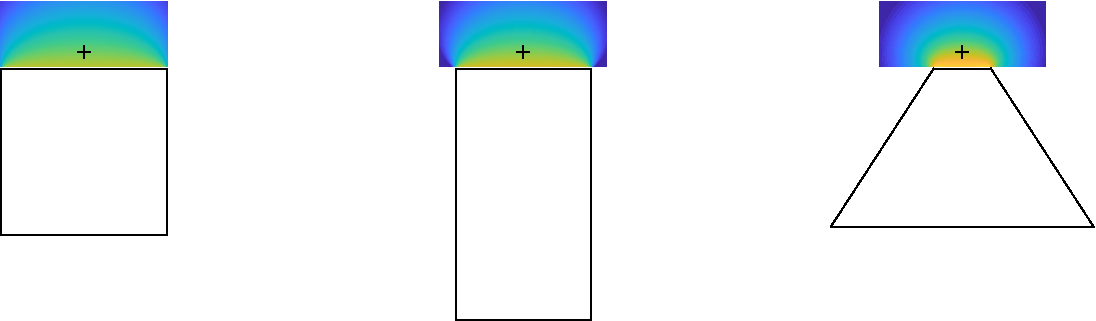
\includegraphics[width=\linewidth]{p3/p3FIG7}
	\caption{The \(z\)-field in the region above a cube magnet, the optimal cuboid magnet, and the optimal frustum magnet for \(z/\upsilon = 0.1\). The point \(z/\upsilon = 0.1\) is drawn with a `+', showing that the optimal frustum magnet gives the strongest field at this point.}
	\label{fig:p3optimalFrusAndCube}
\end{figure*}

An interior-point optimisation algorithm was used to calculate the optimal frustum geometry for a large range of distances \(z/\upsilon\) above the magnet. The optimal parameters \(h_\text{opt}/\upsilon\) and \(\theta_\text{opt}\) were calculated at each \(z/\upsilon\) and are plotted in Figure \ref{fig:p3optimalFrustumGeometry}. As \(z/\upsilon\) increases, the optimal height \(h_\text{opt}/\upsilon\) shows a decreasing trend and the wall angle \(\theta_\text{opt}\) shows an increasing trend. Interestingly, the optimal height \(h_\text{opt}/\upsilon < 1\) for all values of \(z/\upsilon\), meaning the optimal geometry is always a `flatter' magnet. The magnetic field strength for both optimal frustum and optimal cuboid are plotted in Figure \ref{fig:p3PFIeps}, along with the percentage increase in field strength using the optimal frustum rather than the optimal cuboid. This shows a negligible increase in field strength for large \(z/\upsilon\). However, for small \(z/\upsilon\), the increase in field strength may allow more effective use in applications such as magnetic power transmission, linear vibrating systems, and magnetic latching.
\begin{figure}
	\centering
	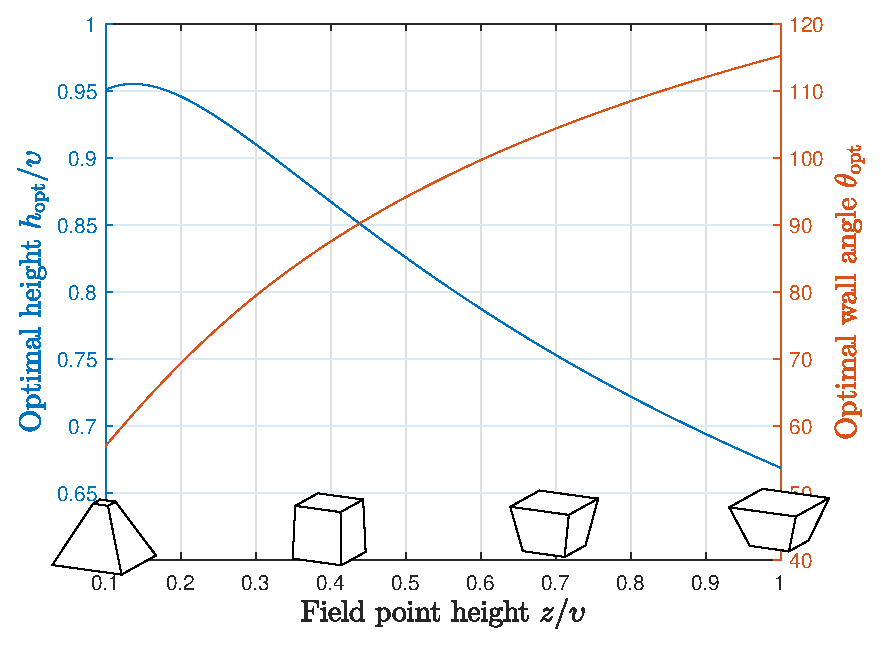
\includegraphics[width=0.8\textwidth]{p3/p3FIG8}
	\caption{Optimal frustum height \(h_\text{opt}\) (blue) and wall angle \(\theta_\text{opt}\) (orange) to maximise the magnetic field strength a distance \(z/\upsilon\) above a right frustum permanent magnet with a volume of \(V\) units\(^3\). A small image of the optimal frustum geometry is displayed at the bottom of the figure for the values \(z/\upsilon =\ \)0.1, 0.4, 0.7, and 1.0.}
	\label{fig:p3optimalFrustumGeometry}
\end{figure}
\begin{figure}
	\centering
	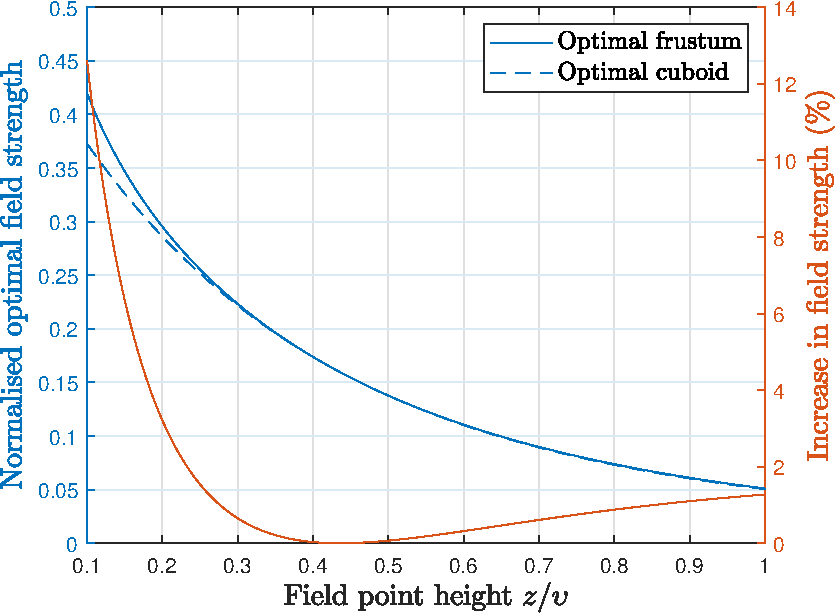
\includegraphics[width=0.8\textwidth]{p3/p3FIG9}
	\caption{Magnetic field strength produced by an optimal frustum and cuboid of the same volume (blue) and percentage increase in the field strength produced by the frustum over the cuboid (orange).}
	\label{fig:p3PFIeps}
\end{figure}
\section{Optimising the field of a planar frustum Halbach array}\label{sec:p3planarArray}
The methods detailed in this paper can also be used to analyse multi-magnet systems. This section focuses on a planar Halbach array created by tessellating frustum magnets for use in planar motors. These arrays may also be used in applications such as planar magnetic loudspeakers and 3D printers. The optimisation routine will vary the geometry to not only increase field strength, but to create a \(z\)-field which closely resembles a desired profile.

\subsection{Defining array geometry}
A planar Halbach array of frustum magnets can be created by tessellating frusta of square-based pyramids and tetrahedra, shown in Figure \ref{fig:p3halbachFrustumGeometry}. Figure \ref{fig:p3halbachFrustumGeometry} shows the repeating unit for this array, which, when duplicated, creates the array shown in Figure \ref{fig:p3planarHalbach}.
\begin{figure*}
	\centering
	\def\Lpontwo{10}
\def\lpontwo{20}
\def\Ltontwo{14}
\def\ltontwo{4}
\def\hh{25}
\def\myscale{0.07}
\def\mywidth{0.3}

\begin{subfigure}[t]{\mywidth\linewidth}

\centering
\tdplotsetmaincoords{70}{35}
\begin{tikzpicture}[scale=\myscale,tdplot_main_coords]

% Define coordinates
\coordinate(1) at (-\Lpontwo,-\Lpontwo,0);
\coordinate(2) at (\Lpontwo,-\Lpontwo,0);
\coordinate(3) at (\Lpontwo,\Lpontwo,0);
\coordinate(4) at (-\Lpontwo,\Lpontwo,0);
\coordinate(5) at (-\lpontwo,-\lpontwo,-\hh);
\coordinate(6) at (\lpontwo,-\lpontwo,-\hh);
\coordinate(7) at (\lpontwo,\lpontwo,-\hh);
\coordinate(8) at (-\lpontwo,\lpontwo,-\hh);

% Draw the shape
\draw (1) -- (2) -- (3) -- (4) -- cycle;
\draw (1) -- (5) -- (6) -- (7) -- (3);
\draw[dashed] (7) -- (8) -- (5);
\draw (2) -- (6);
\draw[dashed] (4) -- (8);

\node(Lp) at (-\Lpontwo-5,3,1) {\(L_p\)};
\node(Lp2) at (0,\Lpontwo+5,1) {\(L_p\)};
\node(lp) at (\lpontwo+5,0,-\hh-1) {\(l_p\)};
\node(lp2) at (3,-\lpontwo-6,-\hh-1) {\(l_p\)};

\end{tikzpicture}

\subcaption{}
\label{subfig:p3pfrus3d}

\end{subfigure}
~
\begin{subfigure}[t]{\mywidth\linewidth}
	
\centering
\tdplotsetmaincoords{70}{35}
\begin{tikzpicture}[scale=\myscale,tdplot_main_coords]

% Define coordinates
\coordinate(1) at (-\Ltontwo,-\Lpontwo,0);
\coordinate(2) at (\Ltontwo,-\Lpontwo,0);
\coordinate(3) at (\Ltontwo,\Lpontwo,0);
\coordinate(4) at (-\Ltontwo,\Lpontwo,0);
\coordinate(5) at (-\ltontwo,-\lpontwo,-\hh);
\coordinate(6) at (\ltontwo,-\lpontwo,-\hh);
\coordinate(7) at (\ltontwo,\lpontwo,-\hh);
\coordinate(8) at (-\ltontwo,\lpontwo,-\hh);

% Draw the shape
\draw (1) -- (2) -- (3) -- (4) -- cycle;
\draw (1) -- (5) -- (6) -- (7) -- (3);
\draw[dashed] (7) -- (8) -- (5);
\draw (2) -- (6);
\draw[dashed] (4) -- (8);

\node(Lp) at (-\Ltontwo-5,3,1) {\(L_p\)};
\node(Lt) at (0,\Lpontwo+5,1) {\(L_t\)};
\node(lp) at (\ltontwo+5,0,-\hh-1) {\(l_p\)};
\node(lt) at (3,-\lpontwo-6,-\hh-1) {\(l_t\)};

\end{tikzpicture}

\subcaption{}
\label{subfig:p3tfrus3d}
	
\end{subfigure}
~
\begin{subfigure}[t]{\mywidth\linewidth}
	
	\centering
	\tdplotsetmaincoords{70}{35}
	\begin{tikzpicture}[scale=0.06,tdplot_main_coords]
	
	% Define coordinates of z frustum
	\coordinate(1z) at (-\Lpontwo,-\Lpontwo,0);
	\coordinate(2z) at (\Lpontwo,-\Lpontwo,0);
	\coordinate(3z) at (\Lpontwo,\Lpontwo,0);
	\coordinate(4z) at (-\Lpontwo,\Lpontwo,0);
	\coordinate(5z) at (-\lpontwo,-\lpontwo,-\hh);
	\coordinate(6z) at (\lpontwo,-\lpontwo,-\hh);
	\coordinate(7z) at (\lpontwo,\lpontwo,-\hh);
	\coordinate(8z) at (-\lpontwo,\lpontwo,-\hh);
	
	% Define coordinates of x frustum
	\coordinate(1x) at (\Lpontwo,-\Lpontwo,0);
	\coordinate(2x) at (\Lpontwo+\Ltontwo+\Ltontwo,-\Lpontwo,0);
	\coordinate(3x) at (\Lpontwo+\Ltontwo+\Ltontwo,\Lpontwo,0);
	\coordinate(4x) at (\Lpontwo,\Lpontwo,0);
	\coordinate(5x) at (\lpontwo,-\lpontwo,-\hh);
	\coordinate(6x) at (\lpontwo+\ltontwo+\ltontwo,-\lpontwo,-\hh);
	\coordinate(7x) at (\lpontwo+\ltontwo+\ltontwo,\lpontwo,-\hh);
	\coordinate(8x) at (\lpontwo,\lpontwo,-\hh);
	
	% Define coordinates of y frustum
	\coordinate(1y) at (-\Lpontwo,\Lpontwo,0);
	\coordinate(2y) at (\Lpontwo,\Lpontwo,0);
	\coordinate(3y) at (\Lpontwo,\Lpontwo+\Ltontwo+\Ltontwo,0);
	\coordinate(4y) at (-\Lpontwo,\Lpontwo+\Ltontwo+\Ltontwo,0);
	\coordinate(5y) at (-\lpontwo,\lpontwo,-\hh);
	\coordinate(6y) at (\lpontwo,\lpontwo,-\hh);
	\coordinate(7y) at (\lpontwo,\lpontwo+\ltontwo+\ltontwo,-\hh);
	\coordinate(8y) at (-\lpontwo,\lpontwo+\ltontwo+\ltontwo,-\hh);
	
	% Deal with certain lines behind objects
	\draw(3y) -- (7y);
	\filldraw[fill=white] (1x) -- (2x) -- (3x) -- (4x) -- cycle;
	\filldraw[fill=white] (2x) -- (3x) -- (7x) -- (6x) -- cycle;
	
	% Draw z frustum
	\draw (1z) -- (2z);
	\draw (3z) -- (4z) -- (1z);
	\draw (1z) -- (5z) -- (6z);
	\draw (2z) -- (6z);
	
	% Draw x frustum
	\draw (5x) -- (6x);
	
	% Draw y frustum
	\draw (2y) -- (3y) -- (4y) -- (1y);
	
	% Draw an invisible node to align left and right pictures
	\node(invis) at (0,0,-1.75*\hh) { };
	
	\end{tikzpicture}
	\subcaption{}
	\label{subfig:p3subarray3d}
	
\end{subfigure}

\begin{subfigure}[t]{\mywidth\linewidth}
	
	\centering
	\begin{tikzpicture}[scale = \myscale]
	
	\coordinate(1) at (-\Lpontwo,0);
	\coordinate(2) at (\Lpontwo,0);
	\coordinate(5) at (-\lpontwo,-\hh);
	\coordinate(6) at (\lpontwo,-\hh);
	
	\draw (1) -- (2) -- (6) -- (5) -- cycle;
	\node(theta) at (-\lpontwo+3,-\hh+2.5) {\(\theta\)};
	\node(Lp) at (0,3.5) {\(L_p\)};
	\node(lp) at (0,-\hh-4) {\(l_p\)};
	\draw[<->] (\lpontwo+5,-\hh) -- (\lpontwo+5,0);
	\node(h) at (\lpontwo+7,-12.5) {\(h\)};
	
	\end{tikzpicture}
	
	\subcaption{}
	\label{subfig:p3pfrusschematic}
	
\end{subfigure}
~
\begin{subfigure}[t]{\mywidth\linewidth}
	
\centering
\begin{tikzpicture}[scale = \myscale]

\coordinate(1) at (-\Ltontwo,0);
\coordinate(2) at (\Ltontwo,0);
\coordinate(5) at (-\ltontwo,-\hh);
\coordinate(6) at (\ltontwo,-\hh);

\draw (1) -- (2) -- (6) -- (5) -- cycle;
\node(theta) at (-\Ltontwo+3,-2.5) {\(\theta\)};
\node(Lp) at (0,3.5) {\(L_t\)};
\node(lp) at (0,-\hh-4) {\(l_t\)};
\draw[<->] (\Ltontwo+5,-\hh) -- (\Ltontwo+5,0);
\node(h) at (\Ltontwo+7,-12.5) {\(h\)};

\end{tikzpicture}

\subcaption{}
\label{subfig:p3tfrusschematic}
	
\end{subfigure}
~
\begin{subfigure}[t]{\mywidth\linewidth}
	
	\centering
	\begin{tikzpicture}[scale=0.055]
	
	% Define coordinates of z frustum
	\coordinate(1z) at (-\Lpontwo,-\Lpontwo);
	\coordinate(2z) at (\Lpontwo,-\Lpontwo);
	\coordinate(3z) at (\Lpontwo,\Lpontwo);
	\coordinate(4z) at (-\Lpontwo,\Lpontwo);
	\coordinate(5z) at (-\lpontwo,-\lpontwo);
	\coordinate(6z) at (\lpontwo,-\lpontwo);
	\coordinate(7z) at (\lpontwo,\lpontwo);
	\coordinate(8z) at (-\lpontwo,\lpontwo);
	
	% Define coordinates of x frustum
	\coordinate(1x) at (\Lpontwo,-\Lpontwo);
	\coordinate(2x) at (\Lpontwo+\Ltontwo+\Ltontwo,-\Lpontwo);
	\coordinate(3x) at (\Lpontwo+\Ltontwo+\Ltontwo,\Lpontwo);
	\coordinate(4x) at (\Lpontwo,\Lpontwo);
	\coordinate(5x) at (\lpontwo,-\lpontwo);
	\coordinate(6x) at (\lpontwo+\ltontwo+\ltontwo,-\lpontwo);
	\coordinate(7x) at (\lpontwo+\ltontwo+\ltontwo,\lpontwo);
	\coordinate(8x) at (\lpontwo,\lpontwo);
	
	% Define coordinates of y frustum
	\coordinate(1y) at (-\Lpontwo,\Lpontwo);
	\coordinate(2y) at (\Lpontwo,\Lpontwo);
	\coordinate(3y) at (\Lpontwo,\Lpontwo+\Ltontwo+\Ltontwo);
	\coordinate(4y) at (-\Lpontwo,\Lpontwo+\Ltontwo+\Ltontwo);
	\coordinate(5y) at (-\lpontwo,\lpontwo);
	\coordinate(6y) at (\lpontwo,\lpontwo);
	\coordinate(7y) at (\lpontwo,\lpontwo+\ltontwo+\ltontwo);
	\coordinate(8y) at (-\lpontwo,\lpontwo+\ltontwo+\ltontwo);
	
	% Draw top plane
	\draw (1z) -- (2z) -- (3z) -- (4z) -- cycle;
	\draw (2y) -- (3y) -- (4y) -- (1y);
	\draw (1x) -- (2x) -- (3x) -- (4x);
	
	% Draw connecting planes where necessary
	\draw (1z) -- (5z);
	\draw (1x) -- (5x) -- (6x) -- (2x);
	\draw (3x) -- (7x) -- (8x) -- (4x);
	\draw (6y) -- (7y) -- (3y);
	\draw (1y) -- (5y) -- (8y) -- (4y);
	
	% Draw bottom plane
	\draw (8z) -- (5z) -- (6z);
	\draw[dashed] (6z) -- (7z) -- (8z);
	\draw[dashed] (7y) -- (8y);
	\draw[dashed] (6x) -- (7x);
	
	% Draw some dimensions
	\draw[<->] (-\Lpontwo,-\lpontwo-5) -- (\Lpontwo,-\lpontwo-5);
	\draw[<->] (\Lpontwo,-\lpontwo-5) -- (\Lpontwo+2*\Ltontwo,-\lpontwo-5);
	\draw[<->] (-\lpontwo-5,-\lpontwo) -- (-\lpontwo-5,\lpontwo);
	\draw[<->] (-\lpontwo-5,\lpontwo) -- (-\lpontwo-5,\lpontwo+2*\ltontwo);
	\node(Lp) at (0,-\lpontwo-10) {\(L_p\)};
	\node(Lt) at (\Lpontwo+\Ltontwo,-\lpontwo-10) {\(L_t\)};
	\node(lp) at (-\lpontwo-9,0) {\(l_p\)};
	\node(lt) at (-\lpontwo-9,\lpontwo+\ltontwo) {\(l_t\)};
	
	\end{tikzpicture}
	\subcaption{}
	\label{subfig:p3subarrayschematic}
	
\end{subfigure}


	\caption{Three dimensional views and schematics of a pyramid frustum (\subref{subfig:p3pfrus3d},\subref{subfig:p3pfrusschematic}), a tetrahedral frustum (\subref{subfig:p3tfrus3d},\subref{subfig:p3tfrusschematic}), and the repeating unit (\subref{subfig:p3subarray3d},\subref{subfig:p3subarrayschematic}).}
	\label{fig:p3halbachFrustumGeometry}
\end{figure*}
\begin{figure}
	\centering
	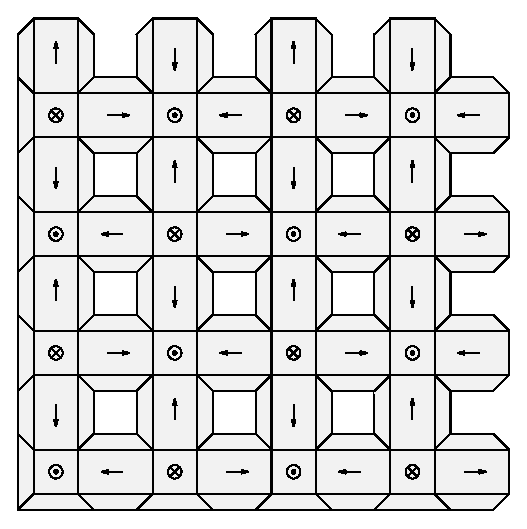
\includegraphics[width=0.7\linewidth]{p3/p3FIG11}
	\caption{Planar Halbach array created by replicating the magnetic subarray from Figure \ref{fig:p3halbachFrustumGeometry}. The pyramid frusta have magnetisations in the \(z\)-direction (into and out of the page), whereas the tetrahedral frusta have magnetisations in the \(x\)- and \(y\)-directions (parallel to the page).}
	\label{fig:p3planarHalbach}
\end{figure}

The square-based pyramid frustum (Figure \ref{fig:p3squareFrustum}) requires three parameters to fully describe its geometry, while the tetrahedral frustum requires five parameters, totalling eight parameters. However, for the magnets to tessellate, two of the length parameters (\(l_p\) and \(L_p\)), the wall angle \(\theta\), and height \(h\) are shared between the two, leaving only four parameters required to fully describe the system geometry. This is reduced to two parameters by keeping the system volume and pole pitch \(\tau\) constant.

Consider the repeating unit shown in Figure \ref{fig:p3halbachFrustumGeometry} (\subref{subfig:p3subarray3d} and \subref{subfig:p3subarrayschematic}) with the magnets having an average volume \(V\). Let the total volume of the three magnets be \(3V\) units\(^3\) and the pole pitch be \(\tau = L_p + L_t = l_p + l_t\) units. Define the parameters \(h\) and \(\theta\) as variables. Thus, the geometry is fully defined by the relations
\begin{align}
l_p &= \tau + h \cot \theta - S \\ 
L_p &= \tau - h \cot \theta - S \\
l_t &= -h \cot \theta + S \\
L_t &= h \cot \theta + S \text{,}
\end{align}
where
\begin{equation}
S = \sqrt{\tau^2 - \frac{3V}{h} - \frac{h^2}{3} \cot^2\theta} \text{.}
\end{equation}
Therefore, for constant \(V\) and \(\tau\), the array geometry can be fully described using the variables \(h\) and \(\theta\).

\subsection{Optimisation of field for a specific case}\label{sec:p3specificOptimisation}
Consider an array using a repeating unit with length \(\tau/\upsilon = 2\) for use in a planar motor with low force ripple and large maximum force. Selection of a suitable desired field profile depends on coil geometry specific to each motor, but this work considers only permanent magnet geometry, and as such a general sinusoidal profile is chosen as the desired \(z\)-field profile. Further extensions of this work could consider a field profile tailored to a particular motor design. Although force ripple will not be completely removed using a sinusoidal profile, it will be reduced when compared to the field produced by a traditional cuboidal array. In addition, a field profile with a large amplitude will lead to a larger maximum force for the motor. Thus, a sinusoid with large amplitude is chosen as the desired field profile for the optimisation routine. Both the resemblance and amplitude can be quantified using a least squares analysis on calculated field data and the appropriate two-dimensional cosine wave \(f\), given by
\begin{equation}\label{eqn:p3cosineWave}
f\left(x,y\right) = A\cos\left(\frac{\pi x}{\tau}\right)\cos\left(\frac{\pi y}{\tau}\right) \text{,}
\end{equation}
where \(A\) is the amplitude of the sinusoid.

For a given geometry \(\left(h/\upsilon,\theta\right)\) and vertical distance \(z/\upsilon\) from the array, the \(z\)-field was calculated over a \(2\tau/\upsilon\times2\tau/\upsilon\) region across a \(32\times32\) grid of points to include one full wavelength of the magnetic field. This calculation was done using five pole pitches in each direction, giving a large enough array such that end effects were negligible, but maintaining a relatively small calculation time. At each point, \(f\) was calculated, and the sum of squared residuals minimised to give the value of the wave amplitude \(A\). The coefficient of determination \(r^2\) was calculated, giving a measure of similarity between the field data and cosine wave. This process was repeated for a large range of geometries \(\left(\theta, h/\upsilon\right)\), and contour plots drawn for \(r^2\) and \(A\). These plots show the optimal regions to maximise \(r^2\) or \(A\), and are shown for \(z/\upsilon = 0.2\) in Figure \ref{fig:p3planarHalbachData}.
\begin{figure}
	\centering
	\begin{subfigure}{0.8\textwidth}
		\centering
		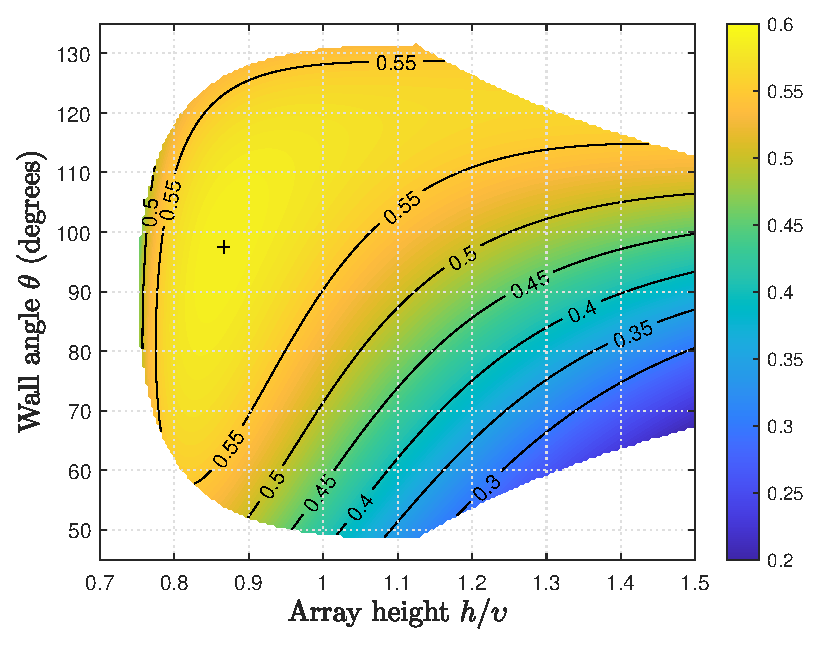
\includegraphics[width=\linewidth]{p3/p3FIG12a}
		\subcaption{}
		\label{subfig:p3planarHalbach_amp}
	\end{subfigure}
	
	\vfill
	
	\begin{subfigure}{0.8\textwidth}
		\centering
		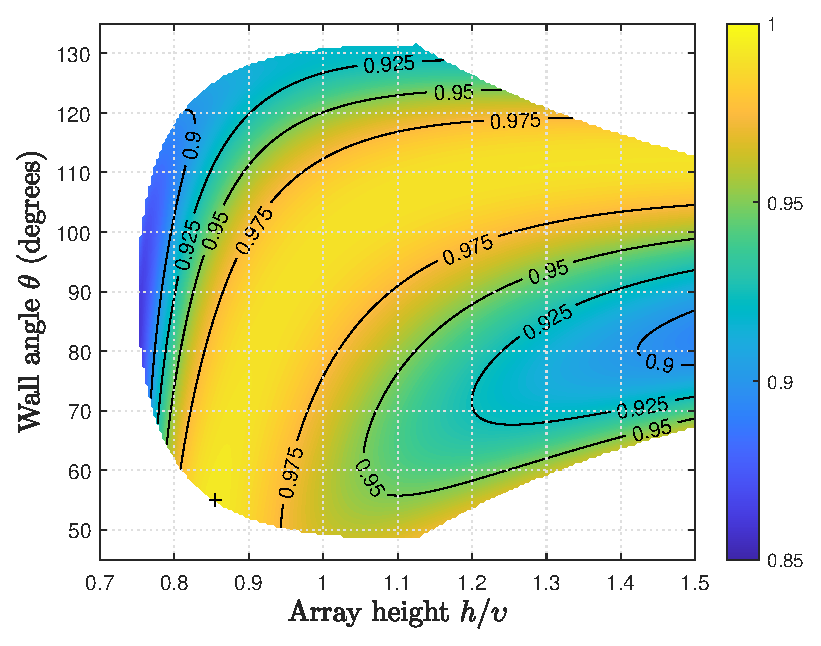
\includegraphics[width=\linewidth]{p3/p3FIG12b}
		\subcaption{}
		\label{subfig:p3planarHalbach_rsq}
	\end{subfigure}
	\caption{Normalised amplitude \(A\) (\subref{subfig:p3planarHalbach_amp}) and coefficient of determination \(r^2\) (\subref{subfig:p3planarHalbach_rsq}) of the cosine wave approximation of the \(z\)-field above the planar magnet array with \(\tau/\upsilon=2\) and \(z/\upsilon = 0.2\). The global maxima are plotted with a `+', with the white region indicating non-physical geometries.}
	\label{fig:p3planarHalbachData}
\end{figure}

The contour plots indicated that there are relatively large regions which maximise \(r^2\) and \(A\). The region to maximise \(r^2\) is a curved stripe, starting with low \(\theta\) and \(h/\upsilon\), passing through the cube case (\(\theta = \) \ang{90}, \(h/\upsilon = 1\)), and tending toward large \(\theta\) and \(h/\upsilon\). The region to maximise \(A\) is a triangular area in the top left of the plot. There is overlap between the optimal regions of both plots along the bottom edge of the optimal region of \(A\) and the top edge of the optimal region of \(r^2\). Hence, the geometry to maximise both \(r^2\) and \(A\) will be in this overlap region.

This can be further examined by defining a cost function to maximise both,
\begin{equation}\label{eqn:p3CostFunction}
C = Ar^2 \text{.}
\end{equation}

Maximising \(C\) will give large values for both \(r^2\) and \(A\), thereby obtaining a field which closely resembles a cosine wave with large amplitude. The cost function \(C\) was calculated at each combination \(\left(\theta, h/\upsilon\right)\) (Figure \ref{fig:p3planarHalbach_wavequality}). This plot shows a region coinciding with the overlap of Figures \ref{subfig:p3planarHalbach_rsq} and \ref{subfig:p3planarHalbach_amp} as expected. The maximum value of this plot occurs at \(h_\text{opt}/\upsilon = 0.89\) and \(\theta_\text{opt} =\) \ang{93.3}. This geometry is almost cuboidal, and thus corresponds to an increase of only 0.04\% in \(C\) over the optimal cuboidal geometry.
\begin{figure}
	\centering
	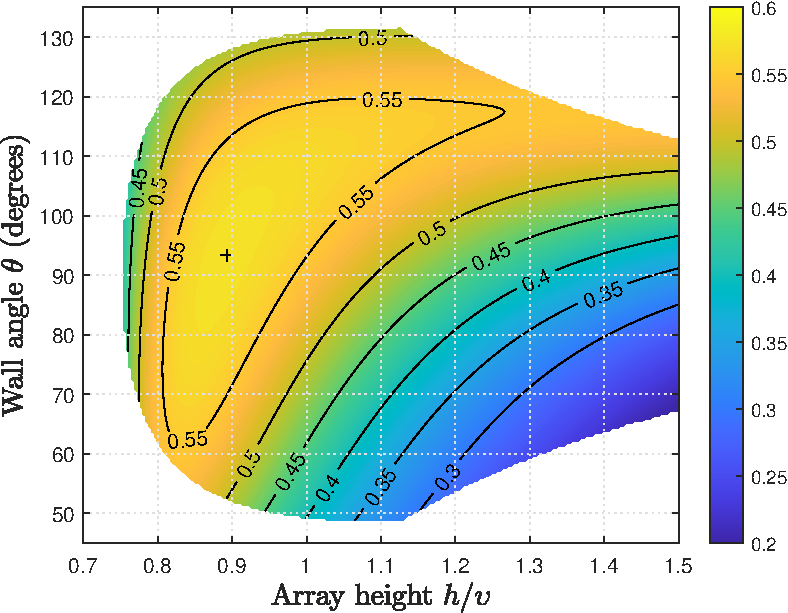
\includegraphics[width=0.8\linewidth]{p3/p3FIG13}
	\caption{The value of the cost function \(C = Ar^2\) at each point in the physically realisable region with \(\tau/\upsilon=2\) and \(z/\upsilon = 0.2\). This value is maximised in the top-left area of the region, with optimal parameters of \(h_\text{opt}/\upsilon = 0.89\) and \(\theta_\text{opt} = \) \ang{93.3}.}
	\label{fig:p3planarHalbach_wavequality}
\end{figure}

\subsection{Optimisation of field for a general case}
The methodology outlined in Section \ref{sec:p3specificOptimisation} can be extended to consider more general cases. However, rather than evaluating the value of \(C\) at each feasible geometry \(\left( \theta, h/\upsilon \right)\), an optimisation routine is used, substantially reducing the number of evaluations of \(C\). Additionally, all length parameters can be normalised by \(z\), allowing a nondimensional analysis, leading to a more general solution.

A range of values were defined for \(\upsilon/z\) and \(\tau/z\), and limits on geometries imposed to discard geometries with extreme aspect ratios. For each combination \(\left( \upsilon/z, \tau/z\right)\), the region of physically realisable geometries was identified in terms of \(h/z\) and \(\theta\). The Matlab function \texttt{fmincon} was then used to maximise the cost function \(C\) over the physically realisable magnet geometries \(\left(\theta, h/z\right)\). This process was repeated for each combination \(\left( \upsilon/z, \tau/z\right)\), and the results plotted on the contour plots in Figure \ref{fig:p3optvalues}, with the corresponding value of the cost function \(C\) plotted in Figure \ref{fig:p3generalPlanarHalbachQuality}.
\begin{figure}
	\centering
	\begin{subfigure}{0.8\textwidth}
		\centering
		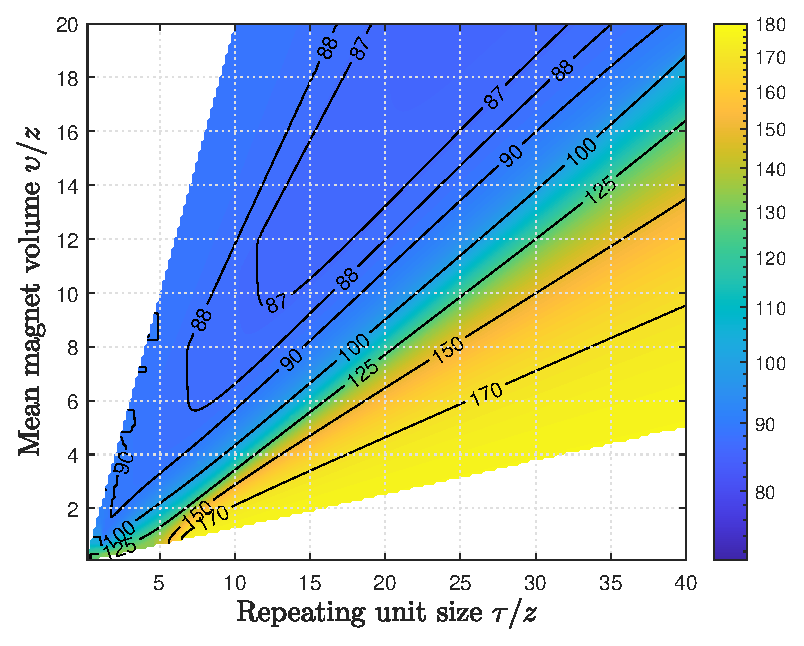
\includegraphics[width=\linewidth]{p3/p3FIG14a}
		\subcaption{}
		\label{subfig:p3opttheta}
	\end{subfigure}
	
	\begin{subfigure}{0.8\textwidth}
		\centering
		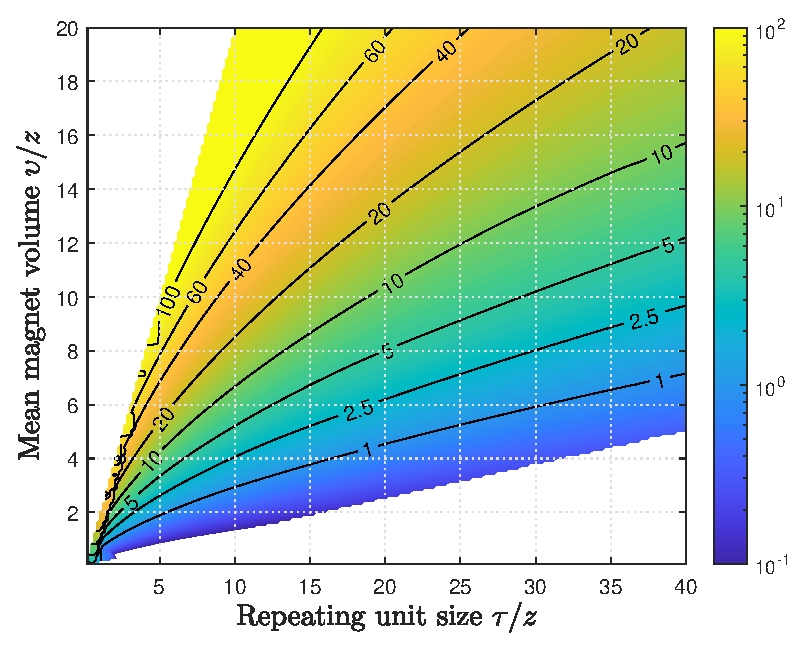
\includegraphics[width=\linewidth]{p3/p3FIG14b}
		\subcaption{}
		\label{subfig:p3opth}
	\end{subfigure}
	\caption{The optimal value of \(\theta\) (\subref{subfig:p3opttheta}) and \(h/z\) (\subref{subfig:p3opth}) for a given combination \(\left( \upsilon/z, \tau/z \right)\). The white regions indicate magnet topologies with undesirable aspect ratios.}
	\label{fig:p3optvalues}
\end{figure}
\begin{figure}
	\centering
	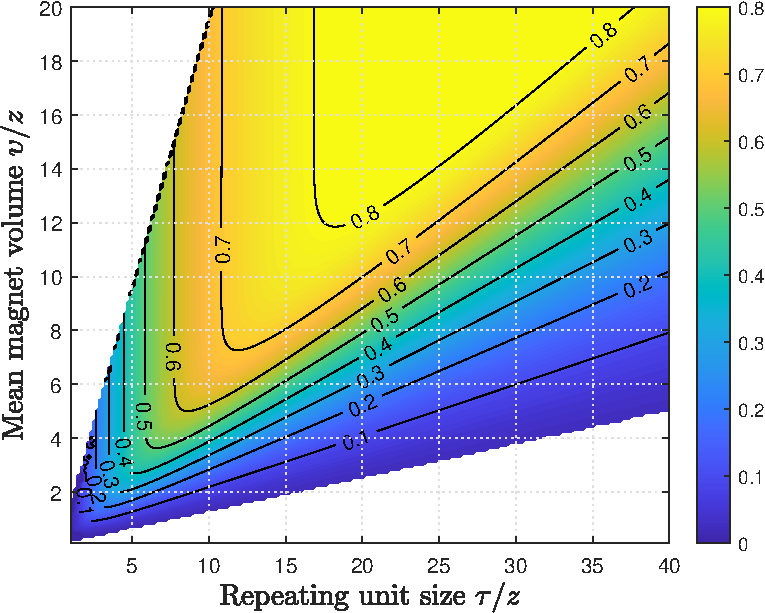
\includegraphics[width=0.8\linewidth]{p3/p3FIG15}
	\caption{The value of the cost function \(C = Ar^2\) at each combination \(\left( \upsilon/z, \tau/z \right)\) normalised by the magnetisation strength of the magnets. This value approaches unity for large \(\tau/z\) and \(\upsilon/z\), and becomes small when either \(\tau/z\) or \(\upsilon/z\) are small.}
	\label{fig:p3generalPlanarHalbachQuality}
\end{figure}

Interestingly, the upper half of the plots indicate a magnet geometry close to a cuboid. However, as the volume decreases or pole pitch increases, the optimal angle \(\theta\) grows larger, leading to a highly non-cuboidal geometry. The optimal height parameter behaves as would be expected, with increasing height as the volume increases or pole pitch decreases.

The optimal frustum topologies can be directly compared to the corresponding cuboidal topologies. The optimisation routine was run again, but this time only optimising the height parameter while maintaining the angle \(\theta\) at \ang{90}. The cost function \(C_\text{cuboid}\) was calculated and compared to the associated frustum cost function \(C\). The percentage increase in \(C\) produced by the optimal frustum over optimal cuboid was plotted for each combination \(\left( \upsilon/z, \tau/z \right)\) and is shown in Figure \ref{fig:p3percentageIncrease}, showing a small but nonzero increase in field quality.
\begin{figure}
	\centering
	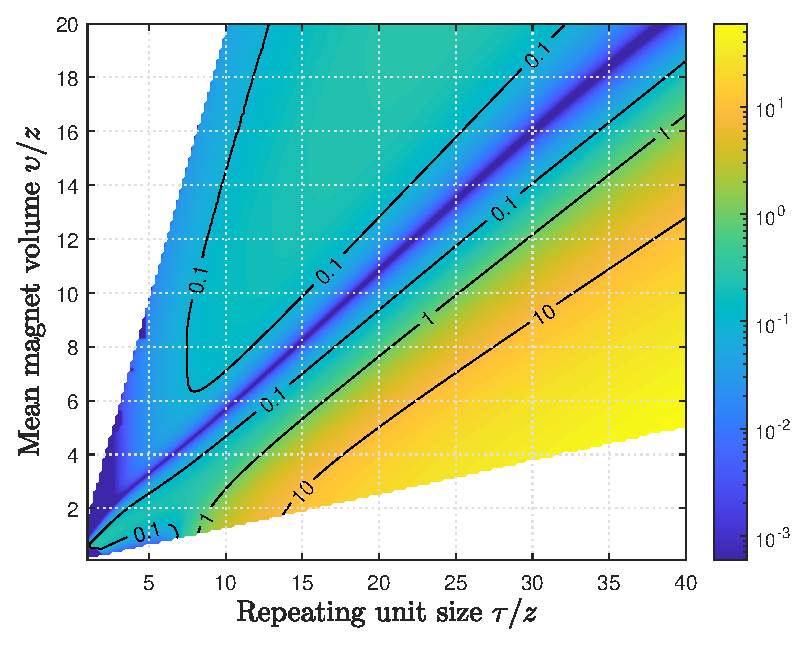
\includegraphics[width=0.8\linewidth]{p3/p3FIG16}
	\caption{Percentage increase in the cost function \(C\) using optimal frustum magnets rather than optimal cuboid magnets. In the centre of the region, the percentage increase is extremely small, implying no effective increase in performance using optimal frusta instead of optimal cuboids. In some regions, this percentage increase is larger. However, these are regions where the cost function is relatively small whether using frusta or cuboids, so it is likely more effective to redesign the system than to optimise magnet geometry.}
	\label{fig:p3percentageIncrease}
\end{figure}

In most of the region, this increase is less than 1 percent, meaning the increased difficulty and cost associate with manufacturing frustum magnets rather than cuboidal magnets is likely not worth the small increase in \(C\). The bottom right region of the plot shows a more considerable percentage increase, achieving an increase greater than 10\%. However, there are two main issues with this region. Firstly, the magnets will exhibit an extremely undesirable aspect ratio. Based on Figure \ref{subfig:p3opth}, this region has a relatively small optimal height parameter \(h/z\) in a region with large \(\tau/z\), leading to a large value of \(\tau/h\) and an undesirable aspect ratio of the magnets. Secondly, this region attains a relatively low value of \(C\) according to Figure \ref{fig:p3generalPlanarHalbachQuality}. This is partially because the magnets are very thin due to the large value of \(\tau/h\), leading to weak fields, and partially because the ratio \(\tau/z\) is large, leading to the field resembling a square wave rather than a sinusoid. These tendencies lead to a small field amplitude \(A\), with a low coefficient of determination \(r^2\), leading to a small value of \(C\).

Based on Figure \ref{fig:p3percentageIncrease}, optimal frustum magnets are likely not worth the additional difficulty and cost associated with manufacturing and assembly for a planar Halbach array. The increase in field amplitude and resemblance to a sinusoid are negligible in most regions. In the region where the increase is not insignificant, the amplitude and resemblance to a sinusoid are small independent of the magnet shape. In this region, it is likely better to redesign the system to increase the magnet volume or decrease the pole pitch of the array. In general, optimal cuboidal magnets are likely the most effective solution for a planar Halbach array which aims to attain a sinusoidal magnetic field with a large amplitude.
\section{Conclusion}\label{sec:p3conclusion}
This paper has examined the differences in the magnetic field produced by frustum permanent magnets and cuboidal permanent magnets. This was done by applying magnetic field equations currently available in literature \cite{OConnell2020a} to a six-faced frustum geometry. Two magnetic systems were considered, allowing a direct comparison between cuboidal magnets and six-faced frustum magnets.

The first magnetic system consisted of a single magnet, with the field being computed at a point directly above the centre of the magnet. In this case, it was shown that an optimised frustum magnet can produce a field stronger than that of an optimised cuboid magnet. However, this increase in field strength is only significant when the field point is close to the magnet. As the field point moves further from the magnet, this increase becomes negligible.

The second magnetic system was a two-dimensional Halbach array consisting of tessellated frustum magnets. For this configuration, the amplitude of the field and how closely the field represents a two-dimensional sinusoid defined a cost function \(C\) (to be maximised), which was used to optimise the system. It was found that most optimal frustum geometries were close to cuboidal. As a comparison, the optimal cuboidal arrays were found, showing that in most cases, the optimal frustum topology has negligible effect on the cost function \(C\). Under certain conditions, the optimal frustum array leads to a significant increase in \(C\) over the optimal cuboid array. However, these conditions lead to a relatively weak field, and other measures should be taken to increase \(C\) such as increasing magnet volume or decreasing the array pole pitch.

This paper shows that although frustum magnets can produce more desirable magnetic fields than cuboidal magnets, this effect is insignificant in many cases. Additionally, complicated magnet geometries such as frusta are more expensive to produce than simple geometries such as cuboids. Hence, the cost associated with the manufacture of these magnets is likely not worth the advantage of a more desirable field. Measures such as varying magnet volume and size are likely to be more effective than using complicated magnet geometries. Furthermore, for multi-magnet arrays, optimising magnet topology and magnetisations is likely more effective than varying the geometry of individual magnets.
\clearpage
\section*{Author's remarks on Chapter \ref{chap:paper3}}
This chapter demonstrated the optimisation of both a singular magnet and a planar array of magnets. For the singular magnet case, the geometry was varied to maximise the magnetic field strength at a point above the centre of the magnet. In the case of the planar magnet array, the array geometry was varied to maximise a cost function associated with the magnetic field above the array. The cost function chosen was a simple two-dimensional sinusoidal pattern, but the choice of cost function has a strong dependence on the application being optimised. Therefore, the results presented in this chapter may not be optimal for every application, but give an indication of the subspace of where the optimal geometry may be. Due to the complexity of the optimisation problem in this chapter, fast field calculation methods such as detailed in Chapter \ref{chap:paper2} were necessary to achieve a solution to the problem in a reasonable time. This chapter has shown a proof of concept in magnetostatic geometry optimisation using efficient field calculations.

\newpage
\section*{References}
\addcontentsline{toc}{section}{\protect\numberline{}References}
\printbibliography[heading=none]